%Service Oriented Computing
\section{Service Oriented Computing}
\label{ServiceOrientedComputing}
This Section gives a brief overview of the Service Oriented domain and its components. We introduce in Section \ref{SOC&SOA} the paradigms to create service oriented infrastructures. Section \ref{WebServices} explains how services can be deployed using the web as media, namely, the Web Services. 
Later in Section \ref{WFManagement} we talk about Workflow management, introducing the terms of Orchestration and Choreography. Right after we dig into the technologies we will be working on throughout the whole project; we overview both BPEL in Section \ref{BPEL} and the remote calls enabled version of Java, Java RMI in Section \ref{JavaRMI}.   

\subsection{Services and composition, SOC and SOA}
\label{SOC&SOA}
During the years preceding the large spread of the Internet, companies used to create their own software systems, in order to obtain highly customized and specific services, rarely focused on the accessibility by external partners.
Today, with the necessity of exchanging information among different companies and businesses, and the push made by the large growth of the Internet, the focus has moved to the integration and the coordination of the existing softwares, namely, the integration of these systems over larger networks.
Defining a \textit{service} as a \textit{"distributed application that exports a view of its functionalities"} \cite{DiLorenzo08}, what is needed is the possibility to compose different services together.
For example, it might be useful to integrate a service (already available on a net), providing maps of a city's streets, with a web-based service listings telephone numbers of a given city zone, resulting in a new service showing telephone numbers directly on a map. %\fxnote{I might add a picture to better show the example here} FIXME
  
The \textit{Service Oriented Computing} (SOC) is the paradigm that attempts to wrap and adapt existing applications into new services, which should comply to three main requirements \cite{DiLorenzo08,Papazoglou03}:
\begin{itemize}
 \item technological independent: the service should be accessible via well known protocols and have a descriptions available on most of the IT environments.
 \item loosely coupled: the client and the provider of the service should not know each other's internal details.
 \item location transparent: clients should be able to get information and access to a service, irrespectively of their location. 
\end{itemize}
Eventually the SOC paradigm makes use of services as the atomic components for developing new applications (which, in turn, can be services too \cite{Papazoglou03}).


To apply the SOC paradigm, there is a need of an architecture infrastructure style, which gives the directives and guidelines to build such a service.  
The architectural infrastructure of the SOC is called \textit{Service Oriented Architecture} (SOA). 
The idea behind the SOA is to describe, publish and make available services (generally speaking, a combination of services) obtained from a preexistent set of applications. 
To achieve the results of making non-homogeneous applications (that use different technologies and run on different platforms) work together, SOA proposes standard interfaces and messaging protocols. This way each of the applications become an atomic, well defined, ready to be connected component. 
The SOA presents an architecture devised in three main components \cite{Pernici04}:
\begin{itemize}
 \item Service provider
 \item Service registry
 \item Service client
\end{itemize}
%as shown in Fig. FIXME: toCreate\ref{fig:The Service Oriented Architecture (SOA)}:
A \textit{service provider}, which makes the service available. The service provider registers its service to the \textit{service registry}, which contains the list of available services and their descriptions. After the registration, the service provider waits for a client to request a service. The service registry can also apply custom access control policies or be entirely public. 
The \textit{service client} contacts the service registry to \textit{find} a service, it gets a contract and the address of the service, making a so called \textit{bind} with the provider. Then it \textit{uses} the service.


Being the realization of services usually based on the reuse of previously existent software, there are many ways to realize it and they can also be combined. For a company, the realization can go from the complete in-house realization to the outsourcing; other options can be to buy/leasing parts of the needed services or to use wrappers/adapters to keep working with the legacy software.
To conclude, from the SOA point of view, services are like black boxes, they can be independently invoked by service clients, without the need of knowing internal details. This makes clients and providers logically decoupled, the client only needs to know the name, the interface and the version of the service. Of course, provider, client and register must be able to use a common communication channel. 

\subsection{Web Services}
\label{WebServices}
We have seen that SOA is an architecture style aimed at the creation of services, though, it does not address the communication channel. \textit{Web Services} (WS) are an instance of a SOA where the communication channel is the web \cite{Pernici04}.
Web services implement the SOA through the application of three main technologies: \textit{SOAP} (Simple Object Access Protocol), \textit{WSDL} (Web Services Description Language) and \textit{UDDI} (Universal Description, Discovery and Integration).
%On the picture of the SOA showed above, we can add these three components.
%, as shown in Fig: (FIXME: to create)\ref{fig:SOA with webServ implement.}.
The SOAP is the web protocol used to exchange messages among the parties. WSDL is the language used by the service provider to fully describe the offered service. At last, UDDI is used by the service registry to make a service easy to find, abstract its technology and make it accessible to the clients.
In the next Subsection we have a brief look into the WSDL technology.

\subsubsection{WSDL (Web Services Description Language) }
\label{Wsdl}
WSDL is a language based on \textit{XML} (eXtensible Markup Language) and it permits to unambiguously describe a web service. For example, it can describe the input parameters a client must provide to use the service and the type of the result the client should expect. 
A WSDL description starts with a \textit{service} tag that identifies a group of related services. Each of the services is then described as following.
The first element is the \verb|port| which identifies the address and the protocol to access the service (e.g. from the IBM online examples \cite{IBMWSDL}: \\
\verb|<soap:address location="http://www.snowbo.../EndorsementSearch"/>|). \\
With \verb|portType|, there are given the specifics of any \verb|operation| that can be used by the client, for example, the input/output parameters or the error messages. The \verb|operation|s comply to one of 4 main patterns: the \verb|One_way| (client sending a message to the provider), the \verb|Request_response| (client sending a message and waiting for an answer form the provider), the \verb|Solicit_response| (Provider sending a message to the client and waiting for a response) and the \verb|Notification| (provider sending a message to the client).
The elements to define the messages and the types used by the service are \verb|message| and \verb|types|. The first specifies the structure of a message to be exchanged. The second, is used to define the atomic types (integer, string, etc.) or new custom types. 
The most important elements in a WSDL service description are summarized in Table \ref{tab:WSDLElements}.

Eventually, we can see that WSDL proposes a static picture of the service. It defines the address and the way to access the service, the operations and, for each of them, the input/output elements to be provided, but it has no notion of the order in which the operations should be called. For example, to access an online shop service, there might be the need to first perform a login operation, check the item availability and last, buy the item. Such an order, or workflow, though, it is not addressed in a WSDL description. This workflow represents the dynamic behavior of a service and it is addressed by the \textit{WorkFlow Management Systems} (WfMS), discussed in the following Section.


% - Who is going to deal with the logic and flow of the composition? \nl 
% - Two main approaches: Orchestration and Choreography, where is the difference \cite{Peltz03} \nl
% - The concept of Workflow management \cite{Aalst98} (picture) and why BPEL is good at it.  \nl
% 
%%%%%%%%%%%%% WSDL TABLE of characteristics %%%%%%%%%%%%%%%%%%%%%%%%%%%%%%%%%%%%%%%%%%%%%%%%%%
\begin{table}
\caption{Basic WSDL elements and their description}
\label{tab:WSDLElements}
\begin{center}
\begin{tabular}{l p{11cm}}

						\toprule
						\addlinespace[0.2cm]
\textbf{WSDL element} 	& \textbf{Description}	\\ 
						\cmidrule(l){1-2}
\verb|port| 		& it identifies the address where the service is found and the protocol to access it 				\\[0,1cm]
\verb|portType| 	& it provides the description of the service, using the \textit{operation} element 				\\[0,1cm]
\verb|operation| 	& it is a basic functionality provided by the service. It lists the input and output messages that are exchanged, in one of the four communication patterns 														\\[0,1cm]
\verb|message| 		& it specifies the format of messages to be exchanged, e.g. the name and type of the variables they contain 	\\[0,1cm]
\verb|types|		& the atomic or user-defined data types in use  								\\[0,1cm]
\verb|binding|		& given a portType, it describes how this is implemented in the specific protocol 				\\[0,1cm]
	 
						\addlinespace[0.2cm]
						\bottomrule
\end{tabular}
\end{center}
\end{table}
%%%%%%%%%%%%%%%%%%%%%%%%%%%%%%%%%%%%%%%%%%%%%%%%%%%%%%%%%%%%%%%%%%%%%%%%%%%%%%%%%%%%%%%%%%%%%%

\subsection{Wf management: Orchestration vs Choreography}
\label{WFManagement}
%This workflow is the dynamic behavior of a service and it is addressed by the \textit{WorkFlow Management Systems} (WfMS), discussed in the following Section.
The workflow description, needed to address the behavior of a web-service is controlled by the \textit{WorkFlow Management Systems} (WfMS). The activities are performed following an execution flow based on four main patterns \cite{Pernici04}: \verb|sequence|, \verb|AND_split|, \verb|OR_split|, \verb|join|. These patterns permit to create generic workflows which are scheduled depending on the availability of the resources.
Two approaches for the workflow management exist: Orchestration and Choreography \cite{Peltz03} explained in the next two paragraphs. Although the two approaches might overlap, their aims differ (see Figure \ref{fig:OrchAndChor}). 

\paragraph{Orchestration}
Orchestration describes the realization of an executable business where the overall control is given to one party. For example, we can show how a travel planner web services orchestrator works (see Figure \ref{fig:orchestration}). Once a client sets the dates and destination of his travel, the travel planner service (coordinator) contacts other three services to book, respectively, a flight, a hotel and a car. The requests and responses to and from the orchestrated services are dealt by the coordinator, which takes care of reporting the found travel information back to the client. These three services can be separated software modules, implemented with different technologies and belonging to different companies.
\paragraph{Choreography}
Choreography also describes the realization of an executable business process, but there is no party having overall control. Here each party collaborates and provides its part and role for the final result. Using the previous example (see Fig. \ref{fig:choreography}), we can notice that the stand alone services have no coordinator. They collaborate exchanging messages among each other. Eventually, choreography takes care of the interactions among the services more than executing a process from one party's perspective.

\subsubsection{Workflow Management for Web Services}
%Among the workflow management systems, there are: FIXME Introduce BPEL and describe it in the next Subsection.
Workflow management systems (WfMS) are computer software dedicated to describe and manage almost any kind of process or job one might think of. For example, WfMS are able to manage a flow of instructions and activities to perform an item manufacturing. When it comes to web services, BPEL (Business Process Execution Language) is surely one of the major characters. BPEL draws its roots in the research made by IBM and Microsoft respectively on WSFL (Web Services Flow Language) and XLANG \cite{Havey2005}. The next Subsection has a deep look into BPEL and its characteristics.

%%%%%%%%%%%%%%%%%FIGURE %%%%%%%%%%%%%%%%%%%%%%%%%%%%%%%%%%55 
 \begin{figure}
\centering
\subfigure[Service orchestration. The travel planner service coordinates the activities of the car rental, flight booking and hotel booking services. ]{
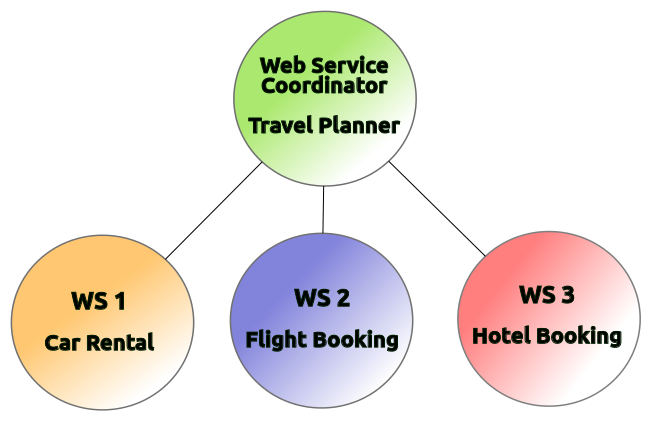
\includegraphics[scale=0.35]{pictures/FigOrchestration}
\label{fig:orchestration}
}
\hspace{2mm}
\subfigure[Service choreography. The services here collaborate to realize the main objective.]{
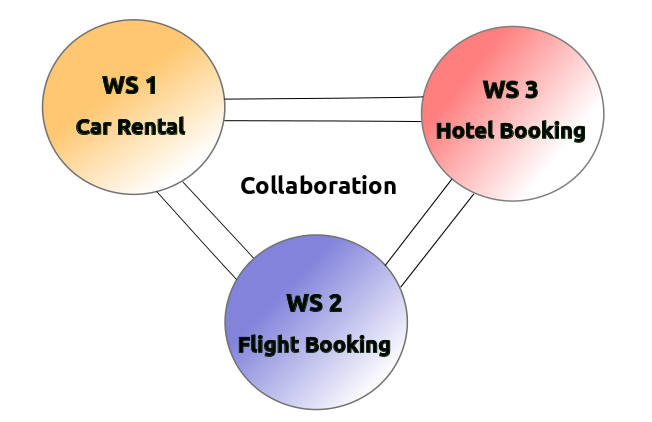
\includegraphics[scale=0.35]{pictures/FigChoreography}
\label{fig:choreography}
}
\caption{Example of service orchestration versus service choreography}
\label{fig:OrchAndChor}
\end{figure} 
%%%%%%%%%%%%%%%%%%%%%%%%%%%%%%%%%%%%%%%%%%%%%%%%%%%%%%%%%%%%%%%

%\subsection{BPEL} FIXME: review!
\subsection{BPEL - The Overview} \label{BPEL}

In today's interconnected world, companies and businesses need to exchange data effectively and get communication flow as fast as possible, in order to save time and be more competitive. They want to automate their business processes and speed up the information exchange. BPEL is a standard that can help them to achieve this goal.
BPEL (which stands for Business Process Execution Language) is an XML standard for describing and defining business processes and hereby standardize the format of information exchange between different softwares. 

BPEL was initially developed by IBM and Microsoft. Its first version (1.0) was released in 2002 by these companies and BEA. Developers wanted to merge IBM's WSFL and Microsoft's XLANG. Both WSFL and XLANG have the same purpose - to combine web services in supporting business processes. During the following year, other companies (Siebel Systems and SAP) joined the development of BPEL and one year later they released version 1.1 together. After this, BPEL was passed to the OASIS nonprofit consortium. In 2007 Web Services BPEL (WS-BPEL) version 2.0 standard was released. During the year 2005 OASIS announced development of extension of WS-BPEL called BPEL4People, including the human interaction in BPEL processes \cite{BPELonWikipedia}.



\paragraph{BPEL Architecture example} \label{BPELarchitecture}
This paragraph contains a brief example of a simple BPEL server and its description. 
In a typical, scenario BPEL process is run on some BPEL engine which is accessible through web services (which among other things contributes to BPEL Architecture platform and operating system independence). After deploying the process, the engine waits for a request (WSDL messages) from clients (which can be for example another BPEL server or a web interface). After the request is received, the BPEL engine creates an instance of a BPEL process and runs it. When running, the process can further interact with the client and also with different BPEL servers. At the end of the operation the result is sent to the client and the process is destroyed in the server.
Note that this is not a general case since BPEL specification does not include any description of the architecture of a BPEL system and therefore this part serves for a reader to get an idea of how BPEL process works (see Figure \ref{BPELprocess}).  

\subsubsection{BPEL Activities} 
\label{BPELActivities}

In a BPEL process, activities are used to define the process logic. Activities are divided into two classes: basic and structured. 

\begin{enumerate}
\item Basic activities are those which describe elementary steps of the process behavior. The following is a list of the most important ones:
	\begin{itemize}
	\item \verb|<invoke>|
	\item \verb|<receive>|
	\item \verb|<reply>|
	\item \verb|<assign>|
	\item \verb|<throw>|
	\end{itemize}

\item Structured activities encode control-flow logic, and can contain other basic and/or structured activities recursively. The most important are listed below:
	\begin{itemize}
	\item \verb|<sequence>|
	\item \verb|<flow>|
	\item \verb|<if>|, \verb|<while>|, \verb|<repeatUntil>|  
	\item \verb|<pick>|
  \end{itemize}
\end{enumerate}


\subsubsection{BPEL Communication}
\label{BPELCommunication}
BPEL processes need to communicate with each other and for this purpose they usually use the combination of a description language, WSDL (see section \ref{Wsdl}), and a protocol, SOAP. WSDL stands for Web Services Description Language and is used to define the interfaces between communicating processes. It means that WSDL determines the format of messages, their data types and types of ports used for transmitting messages \footnote{each port has a particular type(s) assigned and therefore it can receive/send messages of this type(s) only} Whereas WSDL defines the interface between processes, SOAP works on lower level and is used for transmitting the data.

\begin{figure}
\begin{center}
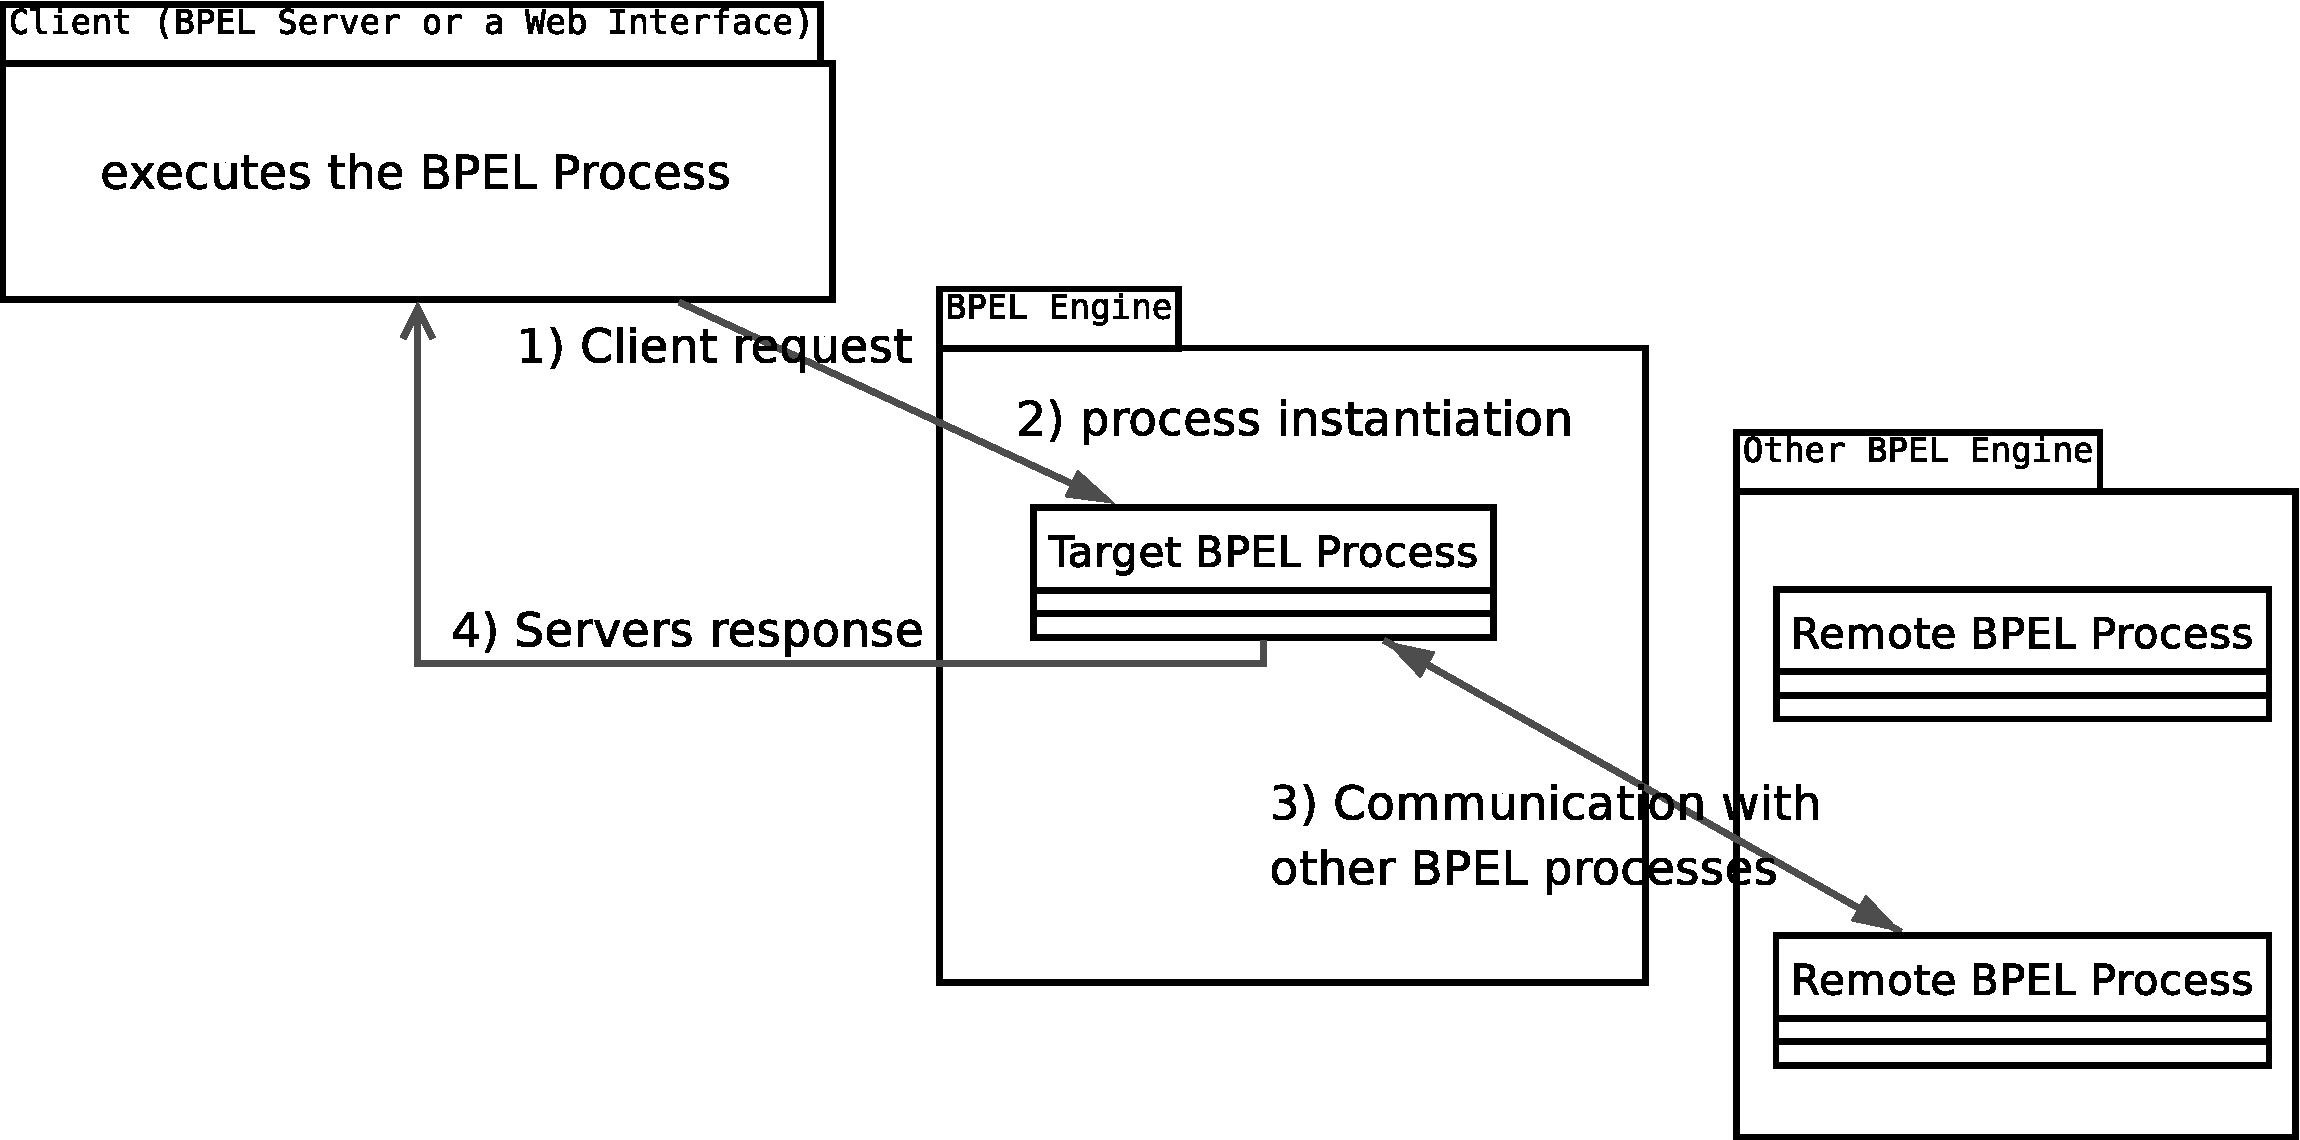
\includegraphics[width=125mm]{pictures/image-BPEL.pdf}
\caption{ Execution of a simple BPEL Process \textbf{FIXME(To Realize with UML Deployment Diagram)}}
\label{BPELprocess}
\end{center}
\end{figure}

\subsubsection{Technologies and protocols used by BPEL}
As mentioned before, BPEL uses WSDL to define process interface and SOAP for message transmitting. On lower levels XML Schema is used for defining the type of XML documents which are sent and received. On the lowest level XML is used for data encapsulation. This can also vary from implementation to implementation. For example, some engines (i.e. Oracle BPEL Process Manager) allow communication with each other using Java RMI instead of SOAP. WS-BPEL 2.0 standard also adds in the specification some new technologies like XPath for accessing data in complex variables and XSLT operations for transforming them \cite{OraBPELRMIInvocation}.


\label{BPELfiles}
BPEL is based on the XML language. As a programming language it has three basic components: the programming logic, the data types and the input/output (I/O). They are divided into three files written in three languages: BPEL, XML Schema definition and WSDL. 
The BPEL file contains the "orchestration" of the system. It specifies an executable process that involves message exchanges between the various processes composing the system. The XML Schema file is used to define the types used in the program. The WSDL file defines the Web Service from an "abstract" point of view describing all the operations for each process participating in the business service.
Table \ref{BPELfilesTable} summarizes the functionalities of the three files composing a BPEL process.

%%%%%%%    Table %%%%%%%%%%%%%%%%%%%%%%%%%%%%%%%%%%%%%%%%%%%%%%
\begin{table}[h!]
\caption{BPEL files' functionalities}
\label{BPELfilesTable}
\begin{center}
\begin{tabular}{l l l}
						\toprule
						\addlinespace[0.2cm]
\textbf{Basic Components} 	& \textbf{Language} 	& \textbf{File extension} 	\\ 
						\cmidrule(l){1-3}
Programming Logic 		& BPEL			& .bpel 			\\[0,1cm]
Data Types 			& XSD (XML Schema) 	& .xsd 				\\[0,1cm]
Input/Output 			& WSDL 			& .wsdl 			\\[0,1cm]
						\addlinespace[0.2cm]
						\bottomrule
\end{tabular}
\end{center}
\end{table}
%%%%%%%%%%%%%%%%%%%%%%%%%%%%%%%%%%%%%%%%%%%%%%%%%%%%%%%%%%%%%%


\paragraph{BPEL Engines}
Table \ref{BPELengines} represents several common BPEL engines developed by various companies \cite{BPELenginesComparisonOnWikipedia}. In this document we do not go deep into the engines' details as we concentrate more on the BPEL process, its orchestration and its functionalities. Of course, sometimes it is not possible to explain BPEL concepts without a basic knowledge about the engines. Thus, brief explanations are provided when necessary.


%%%%%%%%% Table %%%%%%%%%%%%%%%%%%%%%%%%%%%%%%%%%%%%%%%%%%%%%%%%%%%%%%%%%%%
\begin{table}
\caption{List of BPEL engines}
\label{BPELengines}
\begin{center}
\begin{tabular}{l l l}  %\begin{tabular}{|p{5.5cm}|p{3cm}|p{2.5cm}|}
						\toprule
						\addlinespace[0.2cm]
{\bf Name of BPEL Engine} 	& {\bf Supported BPEL Version} 	& {\bf License} 	\\
						\cmidrule(l){1-3}
ActiveBPEL         		& BPEL4WS 1.1, WS-BPEL 2.0 	& GPL and commercial 	\\[0,1cm]
Apache ODE         		& WS-BPEL 2.0 			& Apache license	\\[0,1cm]
jBMP (jBoss)         		& WS-BPEL 2.0 			& LGPL			\\[0,1cm]
Open ESB (Oracle)		& WS-BPEL 2.0 			& Open Source		\\[0,1cm] 
Oracle BPEL Process Manager   	& BPEL4WS 2.0 			& commercial		\\[0,1cm]
WebSphere Process Server (IBM)	& WS-BPEL 2.0			& commercial		\\[0,1cm]
						\addlinespace[0.2cm]
						\bottomrule
\end{tabular}
\end{center}
\end{table}
%%%%%%%%%%%%%%%%%%%%%%%%%%%%%%%%%%%%%%%%%%%%%%%%%%%%%%%%%%%%%%%%%%%%%%%%%%%

%\subsection{Java RMI} FIXME: review!
% Literature review: Summary of Java RMI
% Author: Pierre

\subsection{Java RMI} \label{JavaRMI}   

\textit{Java RMI}, as the name suggests, is an extension of the Java object model, that provides support for distributed objects in the Java language. The remote method calls are done using the same syntax as for local calls, the only difference is that the object making the invocation is aware that its target is remote, as it must handle \textit{RemoteExceptions}. On the other hand, the implementer of a remote object is aware that it is remote because it must implement the \textit{Remote} interface. In order to fill this section we used the Java RMI technology overview \cite{RMI-sun} and the tutorial from the SUN website \cite{RMI-client-sun} and \cite{RMI-overview-sun}.

\paragraph{Remote Interfaces in \textit{Java RMI}}

Remote interfaces are defined by extending an interface called \textit{Remote}, provided in the \textit{java.rmi} package. The remote methods must throw a \textit{RemoteException} in addition to any application specific extension. A remote interface can receive both ordinary and remote objects as arguments, which is also true for its results.

\paragraph{Parameter and result passing}

The arguments of a method are described as \textit{input}, whereas the result is a single \textit{output} parameter. Any object implementing the \textit{serializable} interface (thus being serializable) can be passed as an \textit{input} or \textit{output} in Java RMI.
When the type of a parameter or result value is defined as a remote interface, the corresponding argument or result is always passed as a remote object reference. On the other hand, when a remote object reference is received, it can be used to make RMI calls on the remote object it refers to.
All serializable non-remote objects are copied and passed by value. This way, a new object can be changed locally, possibly causing its state to differ from the one of the original object.

\paragraph{Downloading of classes}

Thanks to Java's virtual machine, classes can easily be transferred from one system to another. This feature is quite useful when placed in the context of distributed objects communicating through remote invocations. If a recipient does not possess the class of an object that has been send to it, the fitting code is downloaded automatically. This allows clients and servers to make transparent use of instances of new classes whenever they are added. Furthermore, there is no need for users to keep the same set of classes in their working environment.

\paragraph{RMI registry}

RMI registry is the middleware in charge of the binding tasks in \textit{Java RMI}. It has to be run on every server hosting remote objects. The RMI registry is actually in charge of maintaining a mapping table associating symbolic object names with remote objects hosted on this computer. It is accessed by methods of the \textit{Naming} class :
\begin{description}
\item[static void 	bind(String name, Remote obj)]
    Binds the specified name to a remote object.
\item[static String[] 	list(String name)]
    Returns an array of the names bound in the registry.
\item[static Remote 	lookup(String name)]
    Returns a reference, a stub, for the remote object associated with the specified name.
\item[static void 	rebind(String name, Remote obj)]
    Rebinds the specified name to a new remote object.
\item[static void 	unbind(String name)]
    Destroys the binding for the specified name that is associated with a remote object.
\end{description}
These methods take a string formatted in the following way as an argument:
\verb|//computerName:port/objectName|
where \textit{computerName} and \textit{port} refer to the location of the RMI registry.
\cite{DS-book}

% New part added by Antonio
% FIXME - I don't know the source of the following text. I need it for citations... I had a look to the "cite" at the beginning of this section, but no source of them fits to it..... :(

\subsubsection{Java RMI Architecture} 
\label{JavaRMIArchitecture}

\paragraph{Interfaces}
\label{JavaRMIinterfaces}
The RMI architecture is based on one important principle: the definition of a behavior and its implementation are separate concepts and their code run on separate JVMs. Moreover, the behavior is described in a Java Interface whereas the implementation is coded in a class \cite{RMI-art5}.
The Java Interface, containing the behavior, runs on the server. There are two implementations of this interface:
\begin{itemize}
	\item On the Server: Behavior's implementation class
	\item On the Client: Proxy class object
\end{itemize}

The client makes method calls directly on the proxy class object, then the proxy sends the request to the server's JVM which contacts the implementation. Any return values are sent back the other way around.

\paragraph{RMI architecture layers}
\label{RMIarchitectureLayers}

\begin{figure}
\begin{center}
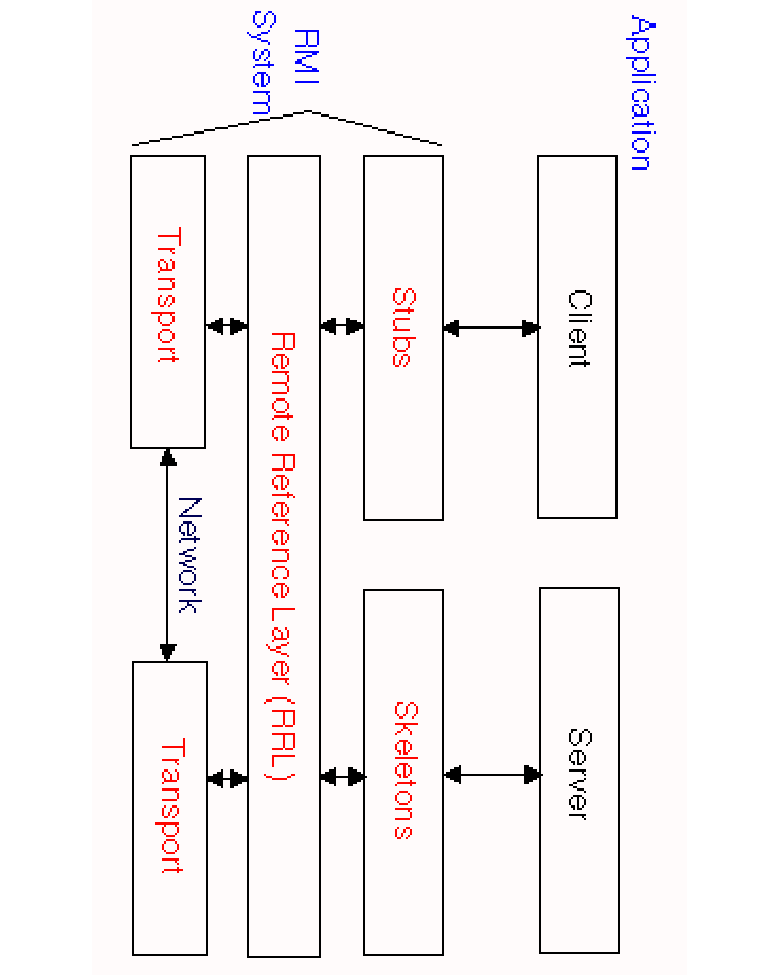
\includegraphics[angle=90, scale=0.65]{pictures/rmi.pdf}
\caption{The layers of RMI}
\label{RMIlayers}
\end{center}
\end{figure}

The RMI implementation is built by three abstract layers shown on Figure \ref{RMIlayers}:

\begin{enumerate}
\item Stub/Skeleton
\item Remote Object Reference
\item Transport Layer
\end{enumerate}

\subparagraph{The Stub and Skeleton layer}
From the client's point of view the Stub object is a proxy which receives all requests directed to the server's service. The Skeleton, on the server side, does almost the same: receives the request from the Stub and passes it to the "real" object containing the method's implementation. Stub and Skeleton don't make any calculation or change on parameters, they just contain the code to communicate to each other. This avoids having to write the implementation of the "communication channel" directly in the client or server Java file. This is why the method's calls look like so similar to local calls. From the JDK 1.2 the Skeleton is not used anymore.
\subparagraph{The Remote Object Reference layer}
The Remote Object Reference layer provides a \verb|RemoteRef| object that represents the link, for the stub, to the class containing the implementation on the server. 
\subparagraph{The transport layer}
The transport layer makes the connection between JVMs and it uses the TCP/IP protocol. Even if two JVMs, containing two different services, are running on the same physical machine, they will connect through the TCP/IP protocol stack. 

%**********************************************************************************

\subsubsection{Java RMI: The Internal Mechanism}
\label{JavaRMIinternalMechanism}

This section concretely explains how Java RMI works and how it can 
help programmers in the writing of the network related code in their programs.

A typical scenario could be: a client wants to execute a method on the server which is on another machine. We will explain why the programmer does not have to write the network and sockets code with Java RMI.

We know that for the service interface on the server, there are two implementations with the same methods: the Stub on the client side and the real object implementing the behavior on the server side. In particular the client uses the stub to call all the methods the same way it would call them on the server. The only difference with a local call is that the stub does not contain the concrete implementation of the required function, it just contains the network-related code to create the communication channel with the server's real implementation \cite{RMI-art4}.
%Thus, from the JDK 1.2, there will be three classes: the client, the stub and the server's real implementation.     
%Client<--->stub<--->[NETWORK]<--->Server_real_implementation.

\paragraph{Socket-Level Details}
\label{SocketLevelDetails}

The following is the list of steps executed by a Java RMI program for each method's call:
\begin{enumerate}
\item The server object listens on an anonymous port on the server machine. The port is chosen at runtime by the JVM or the OS.
\item The client does not know the particular port on the server where the object is listening. It calls the method locally on the stub.
\item The stub creates a TCP/IP communication channel between client and server and it works in 5 steps: 
	\begin{itemize}
	\item The client connects to the server's listening port (see the Bootstrap problem paragraph to understand how the          Stub can know the server's address and port).
  \item The server, waiting for a client's request, accepts the incoming connection and creates a new socket just to 				  handle this single connection.
  \item The server will continue to use the old listening port to wait for other incoming requests.
  \item The communication between client and server takes place using the newly created socket on the server.
  \item They communicate and exchange parameters and results with an agreed-upon protocol. The protocol can be                 \textit{JRMP} (Java Remote Method Protocol) or CORBA-compatible \textit{RMI-IIOP} (Internet Inter-ORB                  Protocol).
	\end{itemize}
\item The method is executed on the server's real implemented object and the result is sent back to the stub.
\item The Stub returns the result back to the client object as if the stub had executed the method locally.
\end{enumerate}

\paragraph{Bootstrap problem}
\label{BootstrapProblem}
In point 2 of paragraph \ref{SocketLevelDetails} we did not explain how the stub on the client side can know the anonymous port where the object is listening on the server. The client has to know at least the IP address of the server machine where the service is available; thus the only problem for the client side is to get the anonymous port.
The RMI registry is used for this purpose: it stays on the server and keeps the correspondences between the name of the service and its address, in a table.
The Registry keeps pairs of $<$public\_name, Stub\_object$>$ in a hashmap, where:
\begin{description}
\item [public\_name] is the name attributed by the server to the implemented object.
\item [Stub\_object] is an instance of the Stub object containing also the address of the anonymous port. 
\end{description}

The following list explains how the Bootstrap problem is solved in Java RMI:
\begin{enumerate}
\item The RMI registry is also a Remote Object and listens on a well-known port on the server machine, by default the 1099.
\item The server creates an object (we call it the \textit{ServiceObject}) listening on an anonymous port.
\item The server automatically creates a \textit{Stub\_ServiceObject} of the new \textit{ServiceObject}
\item When \textit{rebind(String name, Remote obj)} is called on the server side, it passes a Remote Object Reference of the \textit{ServiceObject}, containing the exact port address, as the second parameter. The RMI registry Naming class constructs a new stub object in the registry by copying the already existing \textit{Stub\_ServiceObject} on the server machine and by adding the Remote Object Reference to it.
\item Now there is a pair $<$public\_name, Stub\_object$>$ in the RMI registry containing the name of the service and a Stub object also containing the "real" address of the \textit{ServiceObject} on the server.
\item When the client executes Naming.lookup(public\_name) (e.g \\ Naming.lookup("rmi://Server\_IP\_address:1099/calc") ) it passes the public name as the parameter to the RMI registry on the server. 
\item The RMI registry returns the stored \textit{Stub\_object} object back to the client. Now, the client gets a stub object that knows about the server's host name and port to which the server listens.
\item Now the client can just invoke the \textit{Stub\_object}'s method which will call the same method of the \textit{ServiceObject} on the server.
\end{enumerate}

After all these steps the client and the server don't need the RMI registry anymore. Actually, instead of the Registry, programmers could use different solutions to let the client know about the server's port where the \textit{ServiceObject} is listening, but we will not go into the details of these techniques. 
About the stub, we could say that it is the core of the RMI mechanism. After the Bootstrap it permits programmers to get rid of the communication protocol between client and server and to easily make remote calls like local calls.

%- Overview, features. - Why? it can run everywhere, lightweight scenarios.
%\subsection{Jet}
%\subsection{EMF and Open Architecture Ware (Eclipse)}
%\subsection{other...} 


% %---Where the problem is---
% \subsection{BPEL, its drawbacks and the use of WSs in a lightweight scenario}
% %\subsection{The drawbacks of using BPEL (BPEL and its possible drawbacks)}
% - BPEL, the de-facto standard concerning web services composition. \nl
% - Overview and brief review\nl
% - What do we use of it, the whole language or just a part? \nl %Questo dove andrà??
% - Problems: It works over Distributed Systems, engine powerful but heavy, DS not always available. \nl %i problemi che ha in generale e quelli specifici al nostro caso
% 
% %---Why we face the problem and which is the possible solution (and aim of the work)---
% %\subsection{Web Services Composition in lightweight scenario}
% - That's our question \nl
% - Sometimes we might need services composition working in less powerful environments than distributed systems. Examples? \nl
% - But we don't want to create a new application from scratch neither...(change hardware?).  \nl



